\chapter{System Usage}

\section{Communication Server}

Once the configuration has been completed, navigate to the Follow-Me-Drones/server/ directory and run the following command to run the server:
\begin{itemize}
    \item[\$] python3 comms.py
\end{itemize}

\section{Object Detection}

Once the configuration has been completed, navigate to the Follow-Me-Drones/object-recognition/interface/ directory and run the following commands to open the basic interface:
\begin{itemize}
    \item[\$] \textit{g++ interface.cpp}
    \item[\$] \textit{./a.out}
\end{itemize}

\section{Drone Controls}
If not running a simulation step 1 can be ommited
\begin{itemize}
    \item {Optional} Start Dronekit with the command 
        \newline\textit{\$ dronekit-sitl copter --home=-lat-coords,long-coords,584,353}
    \item Start MavProxy with the command 
        \newline \textbf{\textit{\$ mavproxy.py --master tcp:127.0.0.1:5760 --out udp:127.0.0.1:14551 --out udp:10.1.2.100:14550}}
        \newline --master specifies the IP that the drone commands are supposed to be forward
        \newline --out specifies the ports that can be accessed 
    \item Drone Commands after mavproxy is running
    \begin{itemize}
        \item This is the command to connect to the dronekit.
        \item [] \begin{verbatim}   CONNECT_UDP,UDP_PORT\end{verbatim} 
        \item Disconnects the interface from the drone.
        \item [] \begin{verbatim}   DISCONNECT_UDP\end{verbatim}
        \item Sets the destination for the drone to fly to.
        \item [] \begin{verbatim}   GO_TO_POINT,lat-coords, long-coords\end{verbatim}
        \item Cancels the current flight and sets the drone to return to base.
        \item [] \begin{verbatim}   CANCEL_FLIGHT\end{verbatim}
     \end{itemize}
\end{itemize}

\section{ User Application }
See figure below:
\begin{figure}[h!]
	\centering
	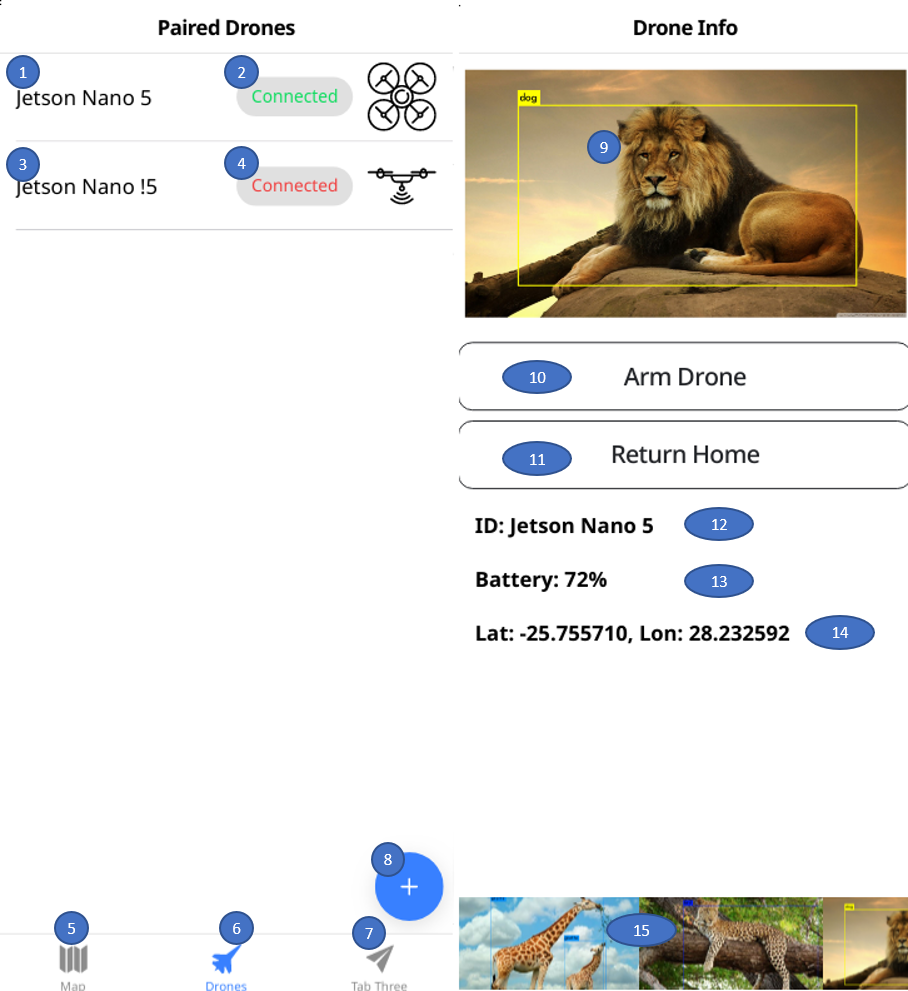
\includegraphics[scale=0.8]{./assets/images/screen.png}
	\label{fig: screens}
	\caption{}
\end{figure}
\begin{itemize}
		\item 1. Device name.
		\item 2. Connection status when drone is connected
		\item 3. Connection status when drone is disconnected
		\item 4. Tab to view map.
		\item 5. Tab to view paired drones
		\item 6. Tab to view current active drone sessions
		\item 7. Pair a new drone.
		\item 8. Currently selected image in carousel below
		\item 9. Arm the drone remotely. (Start object detecttion and lift off)
		\item 10. Return home remotely. (End of session)
		\item 11. Current session. (End of session)
		\item 12. Battery percentage.
		\item 13. Current latitude and longitude coordinates of the drone.
		\item 14. Carousel of previously detected animals.
		
\end{itemize}



